\chapter{Interlude: Cauchy's functional equation and Zorn's lemma}
\label{ch:zorn}
\emph{This is an informal chapter on Zorn's lemma,
which will give an overview of what's going to come in the last parts of the Napkin.
It can be omitted without loss of continuity.}

\medskip

In the world of olympiad math, there's a famous functional equation that goes as follows: 
\[ f : \RR \to \RR \qquad f(x+y) = f(x) + f(y). \]
Everyone knows what its solutions are!
There's an obvious family of solutions $f(x) = cx$.
Then there's also this family of\dots\ uh\dots\ noncontinuous solutions (mumble grumble) pathological 
(mumble mumble) Axiom of Choice (grumble).

There's also this thing called Zorn's lemma. It sounds terrifying,
because it's equivalent to the Axiom of Choice, which is also terrifying because why not.

In this post I will try to de-terrify these things,
because they're really as terrifying as they sound.

\section{Let's construct a monster}
Let us just see if we can try and construct a ``bad'' $f$ and see what happens.

By scaling, let's assume WLOG that $f(1) = 1$.
Thus $f(n) = n$ for every integer $n$, and you can easily show from here that
\[ f\left( \frac mn \right) = \frac mn. \]
So $f$ is determined for all rationals. And then you get stuck.

None of this is useful for determining, say, $f(\sqrt 2)$.
You could add and subtract rational numbers all day
and, say, $\sqrt 2$ isn't going to show up at all.

Well, we're trying to set things on fire anyways, so let's set
\[ f(\sqrt 2) = 2015 \]
because why not?
By the same induction, we get $f(n\sqrt2) = 2015n$, and then that
\[ f\left( a + b \sqrt 2 \right) = a + 2015b. \]
Here $a$ and $b$ are rationals.
Well, so far so good -- as written, this is a perfectly good solution,
other than the fact that we've only defined $f$ on a tiny portion of the real numbers.

Well, we can do this all day:
\[ f\left( a + b \sqrt 2 + c \sqrt 3 + d \pi \right) = a + 2015b + 1337c - 999d. \]
Perfectly consistent.

You can kind of see how we should keep going now.
Just keep throwing in new real numbers which are ``independent''
to the previous few, assigning them to whatever junk we want.
It feels like it \emph{should} be workable. . .

In a moment I'll explain what ``independent'' means (though you
might be able to guess already), but at the moment there's a bigger issue:
no matter how many numbers we throw, it seems like we'll never finish.
Let's address the second issue first.

\section{Review of finite induction}
When you do induction, you get to count off $1$, $2$, $3$, \dots and so on.
So for example, suppose we had a ``problem'' such as:
\begin{quote}
	Prove that the intersection of $n$ open intervals is either $\varnothing$
	or an open interval.
\end{quote}
You can do this by induction easily: it's true for $n = 2$, and
for the larger cases it's similarly easy.

But you can't conclude from this that \emph{infinitely} many open intervals intersect
at some open interval. Indeed, this is false: consider the intervals
\[
	\left( -1, 1 \right), \quad
	\left( -\frac12, \frac12 \right), \quad
	\left( -\frac13, \frac13 \right), \quad
	\left( -\frac14, \frac14 \right), \quad
	\dots
\]
This \emph{infinite} set of intervals intersects at a single point $\{0\}$!

The moral of the story is that induction doesn't let us reach infinity.
Too bad, because we'd have loved to use induction to help us construct a monster.
That's what we're doing, after all -- adding things in one by one.

\section{Transfinite induction}
Well, it turns out we can, but we need a new notion of number,
the so-called \emph{ordinal number}.
I define these in their full glory in the first two sections of \Cref{ch:ordinal}
(and curious readers are even invited to jump ahead to those two sections),
but for this chapter I won't need that full definition yet.

Here's what I want to say: after all the natural numbers
\[ 0, \; 1, \; \dots, \]
I'll put a \emph{new number} called $\omega$,
the first ordinal greater than all the natural numbers.
After that there's more numbers called
\[\omega+1, \; \omega+2, \; \dots \]
and eventually a number called $2\omega$.

The list goes on:
\[
\begin{aligned}
	0, & 1, 2, 3, \dots, \omega \\
	& \omega+1, \omega+2, \dots, \omega+\omega \\
	& 2\omega+1, 2\omega+2, \dots, 3\omega \\
	& \vdots \\
	& \omega^2 + 1, \omega^2+2, \dots \\
	& \vdots \\
	& \omega^3, \dots, \omega^4, \dots, \omega^\omega
	\dots, \omega^{\omega^{\omega^{\dots}}} \\
\end{aligned}
\]
Pictorially, it kind of looks like this:
\begin{center}
	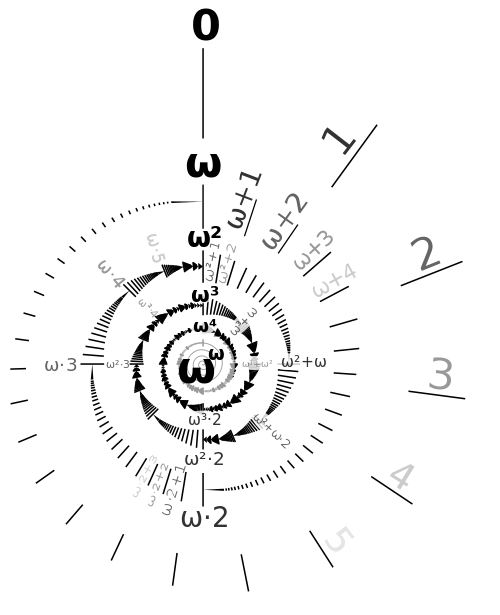
\includegraphics[scale=0.70]{media/500px-Omega-exp-omega-labeled.png}
	\\ \scriptsize Image from \cite{img:omega500}
\end{center}
(Note that the diagram only shows an initial segment;
there are still larger ordinals like $\omega^{\omega^{\omega}}+1000$ and so on).

Anyways, in the same way that natural numbers ``dominate'' all finite sets,
the ordinals dominate \emph{all the sets}, in the following sense.
Essentially, assuming the Axiom of Choice,
it follows that for every set $S$ there's some ordinal $\alpha$
which is larger than $S$ (in a sense I won't make precise until later chapters).

But it turns out (and you can intuitively see) that as large as the ordinals grow,
there is no \emph{infinite descending chain}.
Meaning: if I start at an ordinal (like $2 \omega + 4$) and jump down, I can only
take finitely many jumps before I hit $0$.
(To see this, try writing down a chain starting at $2 \omega + 4$ yourself.)
Hence, induction and recursion still work verbatim:
\begin{theorem}[Transfinite induction]
	Given a statement $P(-)$, suppose that
	\begin{itemize}
		\ii $P(0)$ is true, and
		\ii If $P(\alpha)$ is true for all $\alpha < \beta$, then $P(\beta)$ is true.
	\end{itemize}
	Then $P(\beta)$ is true.
\end{theorem}
Similarly, you're allowed to do recursion to define $x_\beta$ if you know the
value of $x_\alpha$ for all $\alpha < \beta$.

The difference from normal induction or recursion is that we'll often
only do things like ``define $x_{n+1} = \dots$''.
But this is not enough to define $x_\alpha$ for all $\alpha$.
To see this, try using our normal induction and see how far we can climb up the ladder.

Answer: you can't get $\omega$!
It's not of the form $n+1$ for any of our natural numbers $n$ -- our finite induction only lets us
get up to the ordinals less than $\omega$.
Similarly, the simple $+1$ doesn't let us hit the ordinal $2\omega$,
even if we already have $\omega+n$ for all $n$.
Such ordinals are called \vocab{limit ordinals}.
The ordinal that \emph{are} of the form $\alpha+1$ are called \vocab{successor ordinals}.

So a transfinite induction or recursion is very often broken up into three cases.
In the induction phrasing, it looks like
\begin{itemize}
	\ii (Zero Case) First, resolve $P(0)$.
	\ii (Successor Case) Show that from $P(\alpha)$ we can get $P(\alpha+1)$.
	\ii (Limit Case) Show that $P(\lambda)$ holds given $P(\alpha)$ for all $\alpha < \lambda$,
	where $\lambda$ is a limit ordinal.
\end{itemize}
Similarly, transfinite recursion often is split into cases too.
\begin{itemize}
	\ii (Zero Case) First, define $x_0$.
	\ii (Successor Case) Define $x_{\alpha+1}$ from $x_\alpha$.
	\ii (Limit Case) Define $x_\lambda$ from $x_\alpha$ for all $\alpha < \lambda$,
	where $\lambda$ is a limit ordinal.
\end{itemize}
In both situations, finite induction only does the first two cases,
but if we're able to do the third case we can climb far above the barrier $\omega$.

\section{Wrapping up functional equations}
Let's return to solving our problem.

Let $S_n$ denote the set of ``base'' numbers we have at the $n$th step.
In our example, we might have
\[
	S_1 = \left\{ 1 \right\}, \quad
	S_2 = \left\{ 1, \sqrt 2 \right\}, \quad
	S_3 = \left\{ 1, \sqrt 2, \sqrt 3 \right\}, \quad
	S_4 = \left\{ 1, \sqrt 2, \sqrt 3, \pi \right\}, \quad
	\dots
\]
and we'd like to keep building up $S_i$ until we can express all real numbers.
For completeness, let me declare $S_0 = \varnothing$.

First, I need to be more precise about ``independent''.
Intuitively, this construction is working because
\[ a + b \sqrt 2 + c \sqrt 3 + d \pi \]
is never going to equal zero for rational numbers $a$, $b$, $c$, $d$ (other than all zeros).
In general, a set $X$ of numbers is ``independent'' if the combination
\[ c_1 x_1 + c_2 x_2 + \dots + c_m x_m = 0 \]
never occurs for rational numbers $\QQ$ unless $c_1 = c_2 = \dots = c_m = 0$.
Here $x_i \in X$ are distinct. Note that even if $X$ is infinite,
I can only take finite sums!
(This notion has a name: we want $X$ to be \textbf{linearly independent} over $\QQ$;
see the chapter on vector spaces for more on this!)

When do we stop?
We'd like to stop when we have a set $S_{\text{something}}$ that's so big,
every real number can be written in terms of the independent numbers.
(This notion also has a name: it's called a $\QQ$-basis.)
Let's call such a set \textbf{spanning};
we stop once we hit a spanning set.

The idea that we can induct still seems okay:
suppose $S_\alpha$ isn't spanning.
Then there's some number that is independent of $S_\alpha$, say $\sqrt{2015}\pi$ or something.
Then we just add it to get $S_{\alpha+1}$.
And we keep going.

Unfortunately, as I said before it's not enough to be able to go from $S_\alpha$ to $S_{\alpha+1}$
(successor case); we need to handle the limit case as well.
But it turns out there's a trick we can do.
Suppose we've constructed \emph{all} the sets $S_0$, $S_1$, $S_2$, \dots, one for each positive integer $n$,
and none of them are spanning.
The next thing I want to construct is $S_\omega$; somehow I have to ``jump''.
To do this, I now take the infinite union
\[ S_\omega \overset{\text{def}}{=} S_0 \cup S_1 \cup S_2 \cup \dots. \]
The elements of this set are also independent (why?).

Ta-da!
With the simple trick of ``union all the existing sets'',
we've just jumped the hurdle to the first limit ordinal $\omega$.
Then we can construct $S_{\omega+1}$, $S_{\omega+2}$, \dots, once again --
just keep throwing in elements.
Then when we need to jump the next hurdle to $S_{2 \omega}$,
we just do the same trick of ``union-ing'' all the previous sets.

So we can formalize the process as follows:
\begin{enumerate}
	\ii Let $S_0 = \varnothing$.
	\ii For a successor stage $S_{\alpha+1}$, add any element to $S_\alpha$ to obtain $S_{\alpha+1}$.
	\ii For a limit stage $S_{\lambda}$, take the union $\bigcup_{\gamma < \lambda} S_\gamma$.
\end{enumerate}
How do we know that we'll stop eventually?
Well, the thing is that this process consumes a lot of real numbers.
In particular, the ordinals get larger than the size of $\RR$ (assuming Choice).
Hence if we don't stop we will quite literally reach a point where we have used up every single real number.
Clearly that's impossible, because by then the elements can't possibly be independent!

So by transfinite recursion, we eventually hit some $S_\gamma$ which is spanning:
the elements are all independent, but every real number can be expressed using it.
Done!

\section{Zorn's lemma}
Now I can tell you what Zorn's lemma is:
it lets us do the same thing in any poset.

We can think of the above example as follows:
consider all sets of independent elements.
These form a partially ordered set by inclusion, and what we did
was quite literally climb up a chain
\[ S_0 \subsetneq S_1 \subsetneq S_2 \subsetneq \dots. \]
It's not quite climbing since we weren't just going one step at a time:
we had to do ``jumps'' to get up to $S_\omega$ and resume climbing.
But the main idea is to climb up a poset until we're at the very top;
in the previous case, when we reached the spanning set.

The same thing works verbatim with any \href{http://en.wikipedia.org/wiki/Partially_ordered_set}{partially ordered set}
$\mathcal P$.
Let's define some terminology.
A \vocab{local maximum} of the entire poset $\mathcal P$ is an element
which has no other elements strictly greater than it.
(Most authors refer to this as ``maximal element'', but I think
``local maximum'' is a more accurate term.)

Now a \vocab{chain of length $\gamma$} is a set of elements $p_\alpha$ for every $\alpha < \gamma$
such that $p_0 < p_1 < p_2 < \dots$.
(Observe that a chain has a last element if and only if $\gamma$ is a successor ordinal, like $\omega+3$.)
An \vocab{upper bound} to a chain is an element $\tilde p$ which is greater than or equal
to all elements of the chain;
In particular, if $\gamma$ is a successor ordinal, then just taking the last element of the chain works.

In this language, Zorn's lemma states that
\begin{theorem}
	[Zorn's lemma]
	Let $\mathcal P$ be a nonempty partially ordered set.
	If every chain has an upper bound,
	then $\mathcal P$ has a local maximum.
\end{theorem}

Chains with length equal to a successor ordinal always have upper bounds,
but this is not true in the limit case.
So the hypothesis of Zorn's lemma is exactly what
lets us ``jump'' up to define $p_\omega$ and other limit ordinals.
And the proof of Zorn's lemma is straightforward: keep climbing up the poset at successor stages,
using Zorn's condition to jump up at limit stages, and thus building a really long chain.
But we have to eventually stop, or we literally run out of elements of $\mathcal P$.
And the only possible stopping point is a local maximum.

If we want to phrase our previous solution in terms of Zorn's lemma, we'd say:
\begin{proof}
	Look at the poset whose elements are sets of independent real numbers.
	Every chain $S_0 \subsetneq S_1 \subsetneq \dots$ has an upper bound $\bigcup S_\alpha$
	(which you have to check is actually an element of the poset).
	Thus by Zorn, there is a local maximum $S$.
	Then $S$ must be spanning, because otherwise we could add an element to it.
\end{proof}
So really, Zorn's lemma is encoding all of the work of climbing that I argued earlier.
It's a neat little package that captures all the boilerplate, and tells
you exactly what you need to check.

\begin{center}
	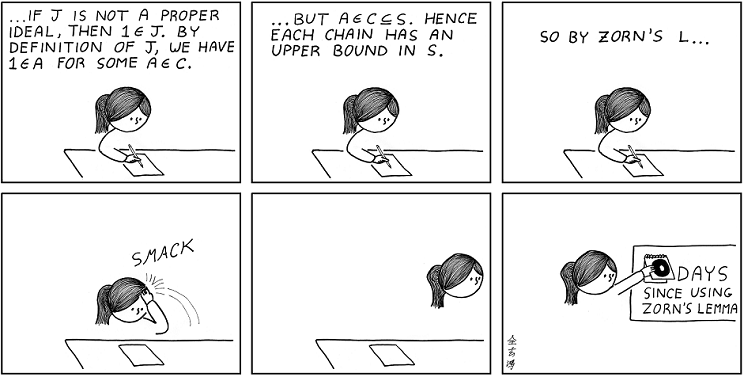
\includegraphics[scale=0.5]{media/zornaholic.png}
	\\ \scriptsize Image from \cite{img:zornaholic}
\end{center}

One last thing you might ask:
where is the Axiom of Choice used?
Well, the idea is that for any chain there could be lots of $\tilde p$'s,
and you need to pick one of them.
Since you are making arbitrary choices infinitely many times, you need the Axiom of Choice.
(Actually, you also need choice to talk about cardinalities as in theorem 1.)
But really, it's nothing special.

\section{\problemhead}
\begin{problem}
	[Tukey's lemma]
	Let $\mathcal F$ be a nonempty family of sets.
	Assume that for any set $A$,
	the set $A$ is in $\mathcal F$
	if and only if all its finite subsets are in $\mathcal F$.

	Prove that there exists a maximal set $Y \in \mathcal F$
	such that $X \subseteq Y$ for every $X \in \mathcal F$.
\end{problem}
